\setcounter{figure}{0}
\setcounter{table}{0}
\renewcommand{\thefigure}{S\arabic{figure}}
\renewcommand{\thetable}{S\Roman{table}}

\section*{Supplemental Material}

\begin{figure*}[h]
  \begin{center}
  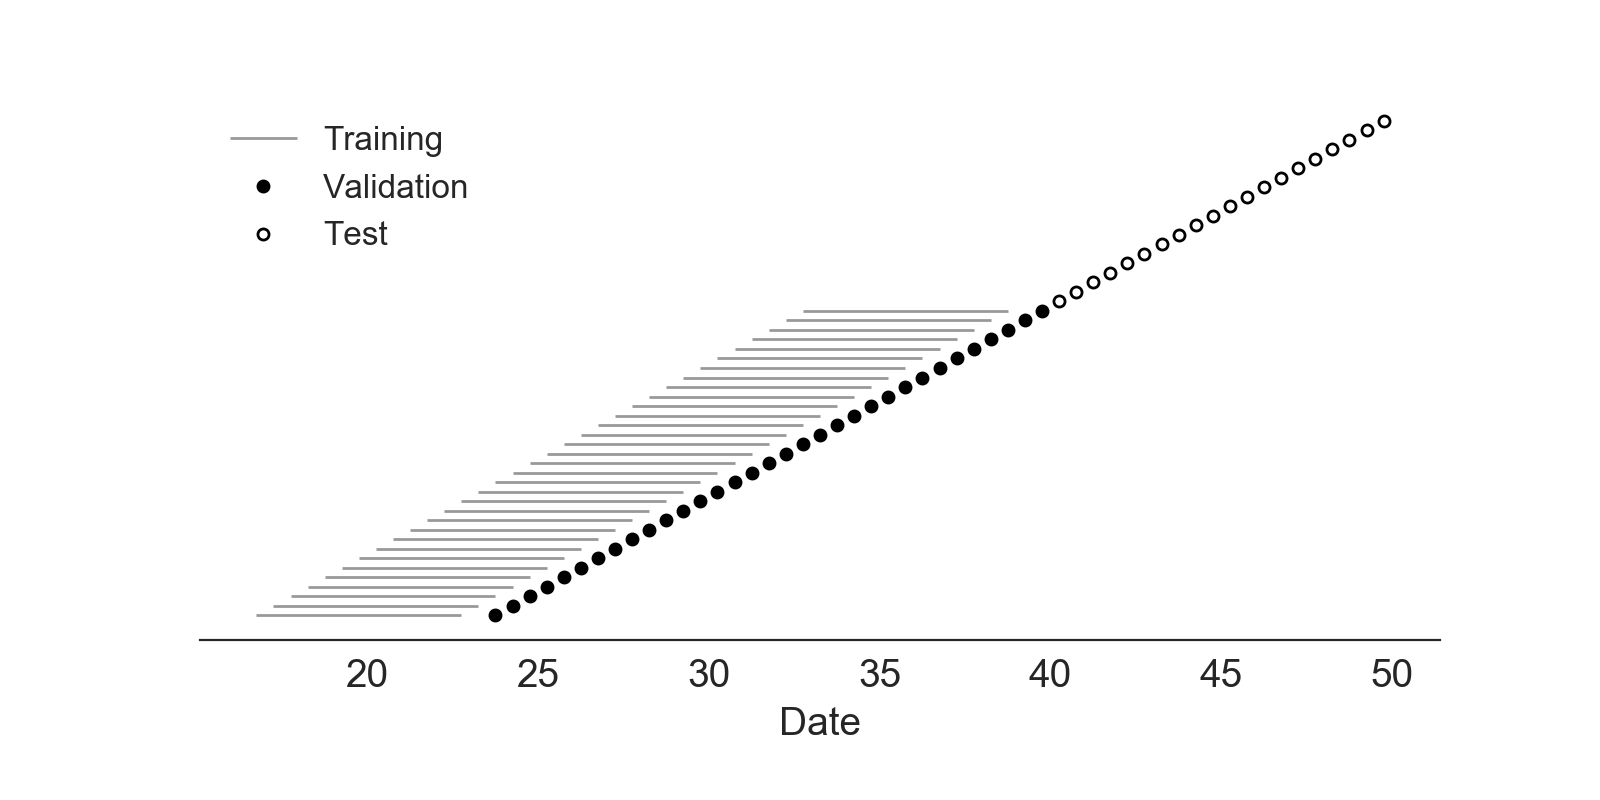
\includegraphics[width=\textwidth]{figures/cross-validation-for-simulated-populations.png}
  \caption{
  Time-series cross-validation scheme for simulated populations.
  Models were trained in six-year sliding windows (grey lines) and validated on out-of-sample data from validation timepoints (filled circles).
  Validation results from 30 years of data were used to iteratively tune model hyperparameters.
  After fixing hyperparameters, model coefficients were fixed at the mean values across all training windows.
  Fixed coefficients were applied to 10 years of new out-of-sample test data (open circles) to estimate true forecast errors.
  }
  \label{sup_fig:cross_validation_for_simulated_populations}
  \end{center}
\end{figure*}

\begin{figure*}[h]
  \begin{center}
  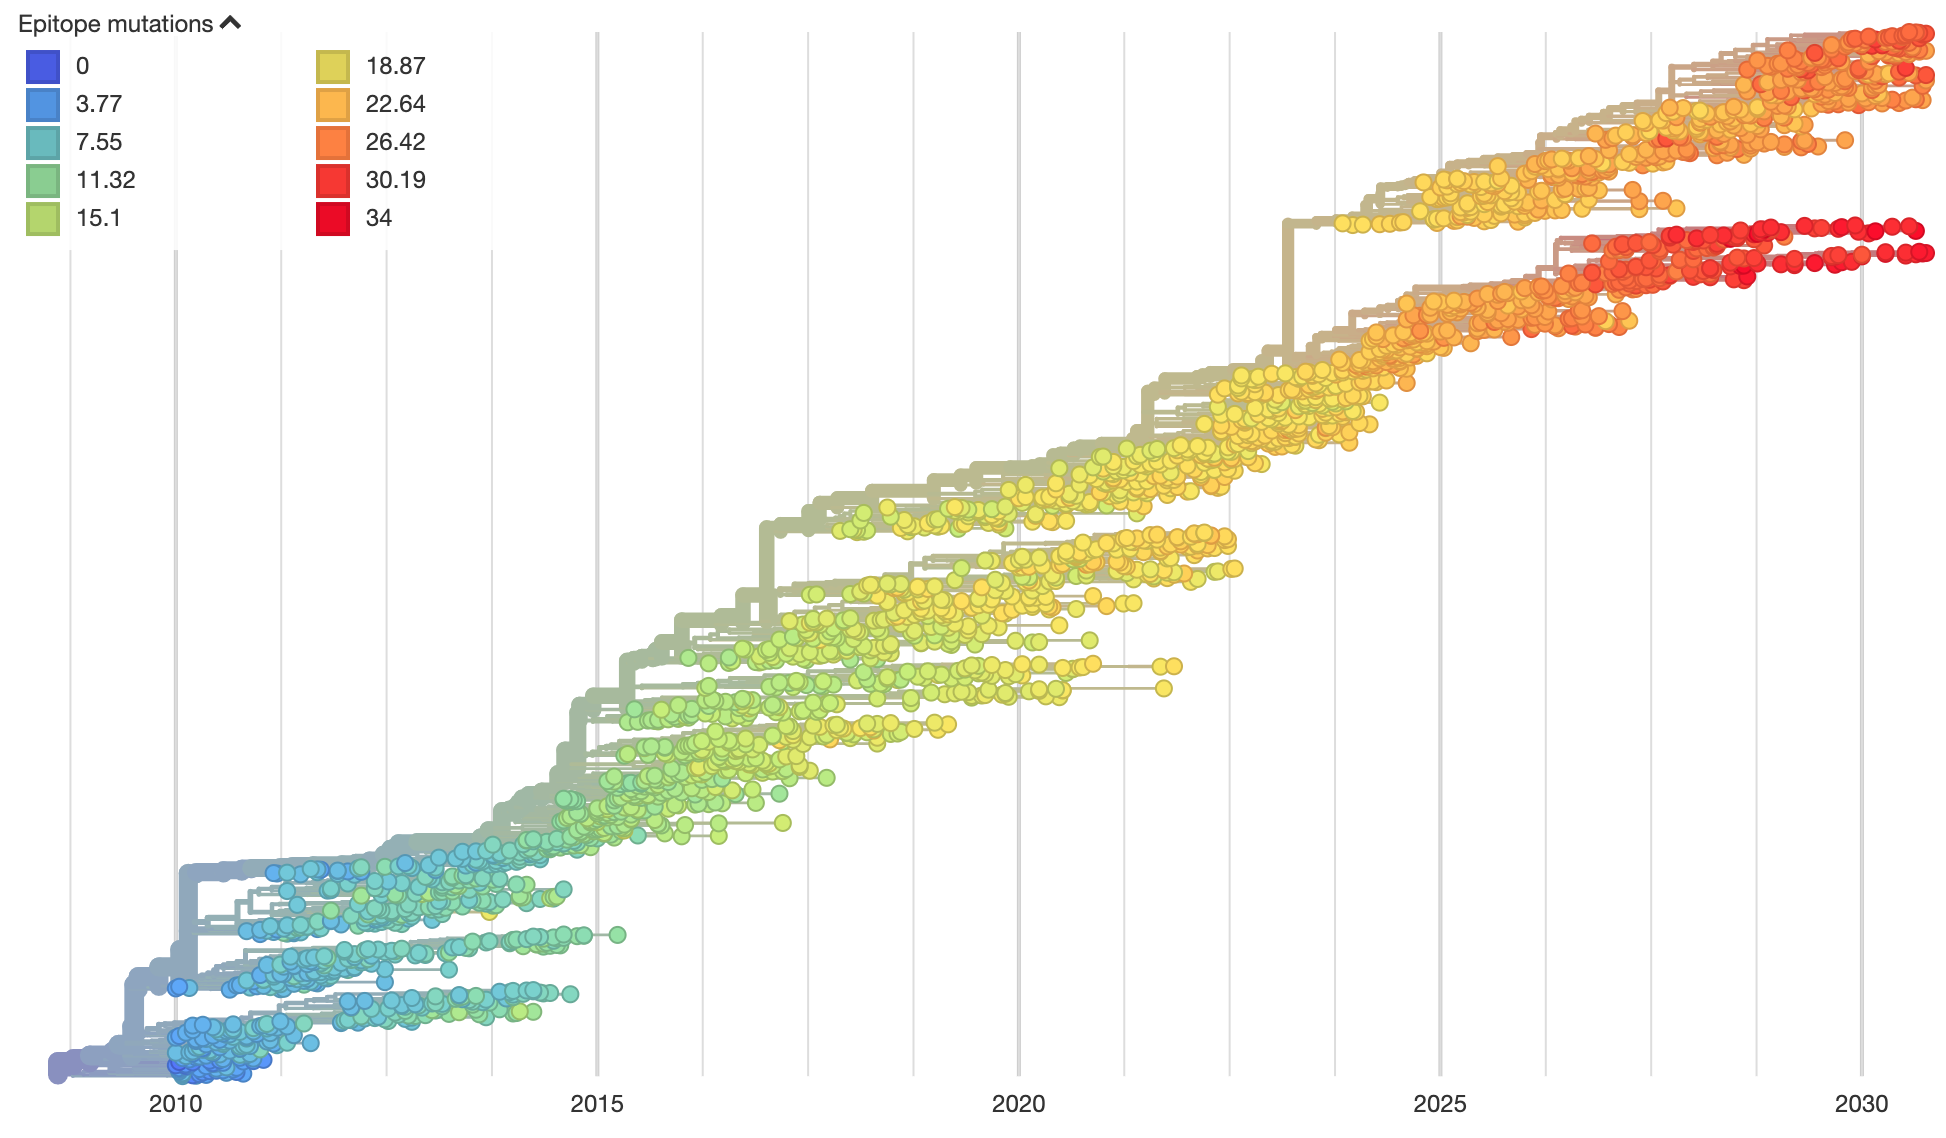
\includegraphics[width=\textwidth]{figures/simulated-h3n2-ha-phylogeny.png}
  \caption{
  Phylogeny of A/H3N2-like HA sequences sampled between the 24th and 30th years of simulated evolution.
  The phylogenetic structure and rate of accumulated epitope and non-epitope mutations match patterns observed in phylogenies of natural sequences.
  Sample dates were annotated as the generation in the simulation divided by 200 and added to 2000, to acquire realistic date ranges that were compatible with our modeling machinery.
  }
  \label{sup_fig:simulated_h3n2_ha_phylogeny}
  \end{center}
\end{figure*}

\begin{table*}[ht]
  \begin{center}
    \begin{tabular}{lrrr}
\toprule
{} &  epitope mutations &  non-epitope mutations &  epitope-to-non-epitope ratio \\
branch type &                    &                        &                               \\
\midrule
side branch &                590 &                   1327 &                          0.44 \\
trunk       &                 23 &                     12 &                          1.92 \\
\bottomrule
\end{tabular}

    \caption{
    Number of epitope and non-epitope mutations per branch by trunk or side branch status for simulated populations.
    Epitope sites were defined previously described \cite{Luksza:2014hj}.
    Annotation of trunk and side branch was performed as previously described \cite{Bedford:2015fj}.
    Mutations were calculated for the full validation tree for simulated sequences samples between October of years 10 and 40.
    }
    \label{sup_table:mutations_by_trunk_status_for_simulated_populations}
  \end{center}
\end{table*}

\begin{table*}[ht]
  \begin{center}
    \begin{tabular}{lrrr}
\toprule
{} &  epitope mutations &  non-epitope mutations &  epitope-to-non-epitope ratio \\
branch type &                    &                        &                               \\
\midrule
side branch &                485 &                   1177 &                          0.41 \\
trunk       &                 50 &                     32 &                          1.56 \\
\bottomrule
\end{tabular}

    \caption{
    Number of epitope and non-epitope mutations per branch by trunk or side branch status for natural populations.
    Epitope sites were defined previously described \cite{Luksza:2014hj}.
    Annotation of trunk and side branch was performed as previously described \cite{Bedford:2015fj}.
    Mutations were calculated for the full validation tree for natural sequences samples between 1990 and 2015.
    }
    \label{sup_table:mutations_by_trunk_status}
  \end{center}
\end{table*}

\begin{figure*}[t]
  \begin{center}
  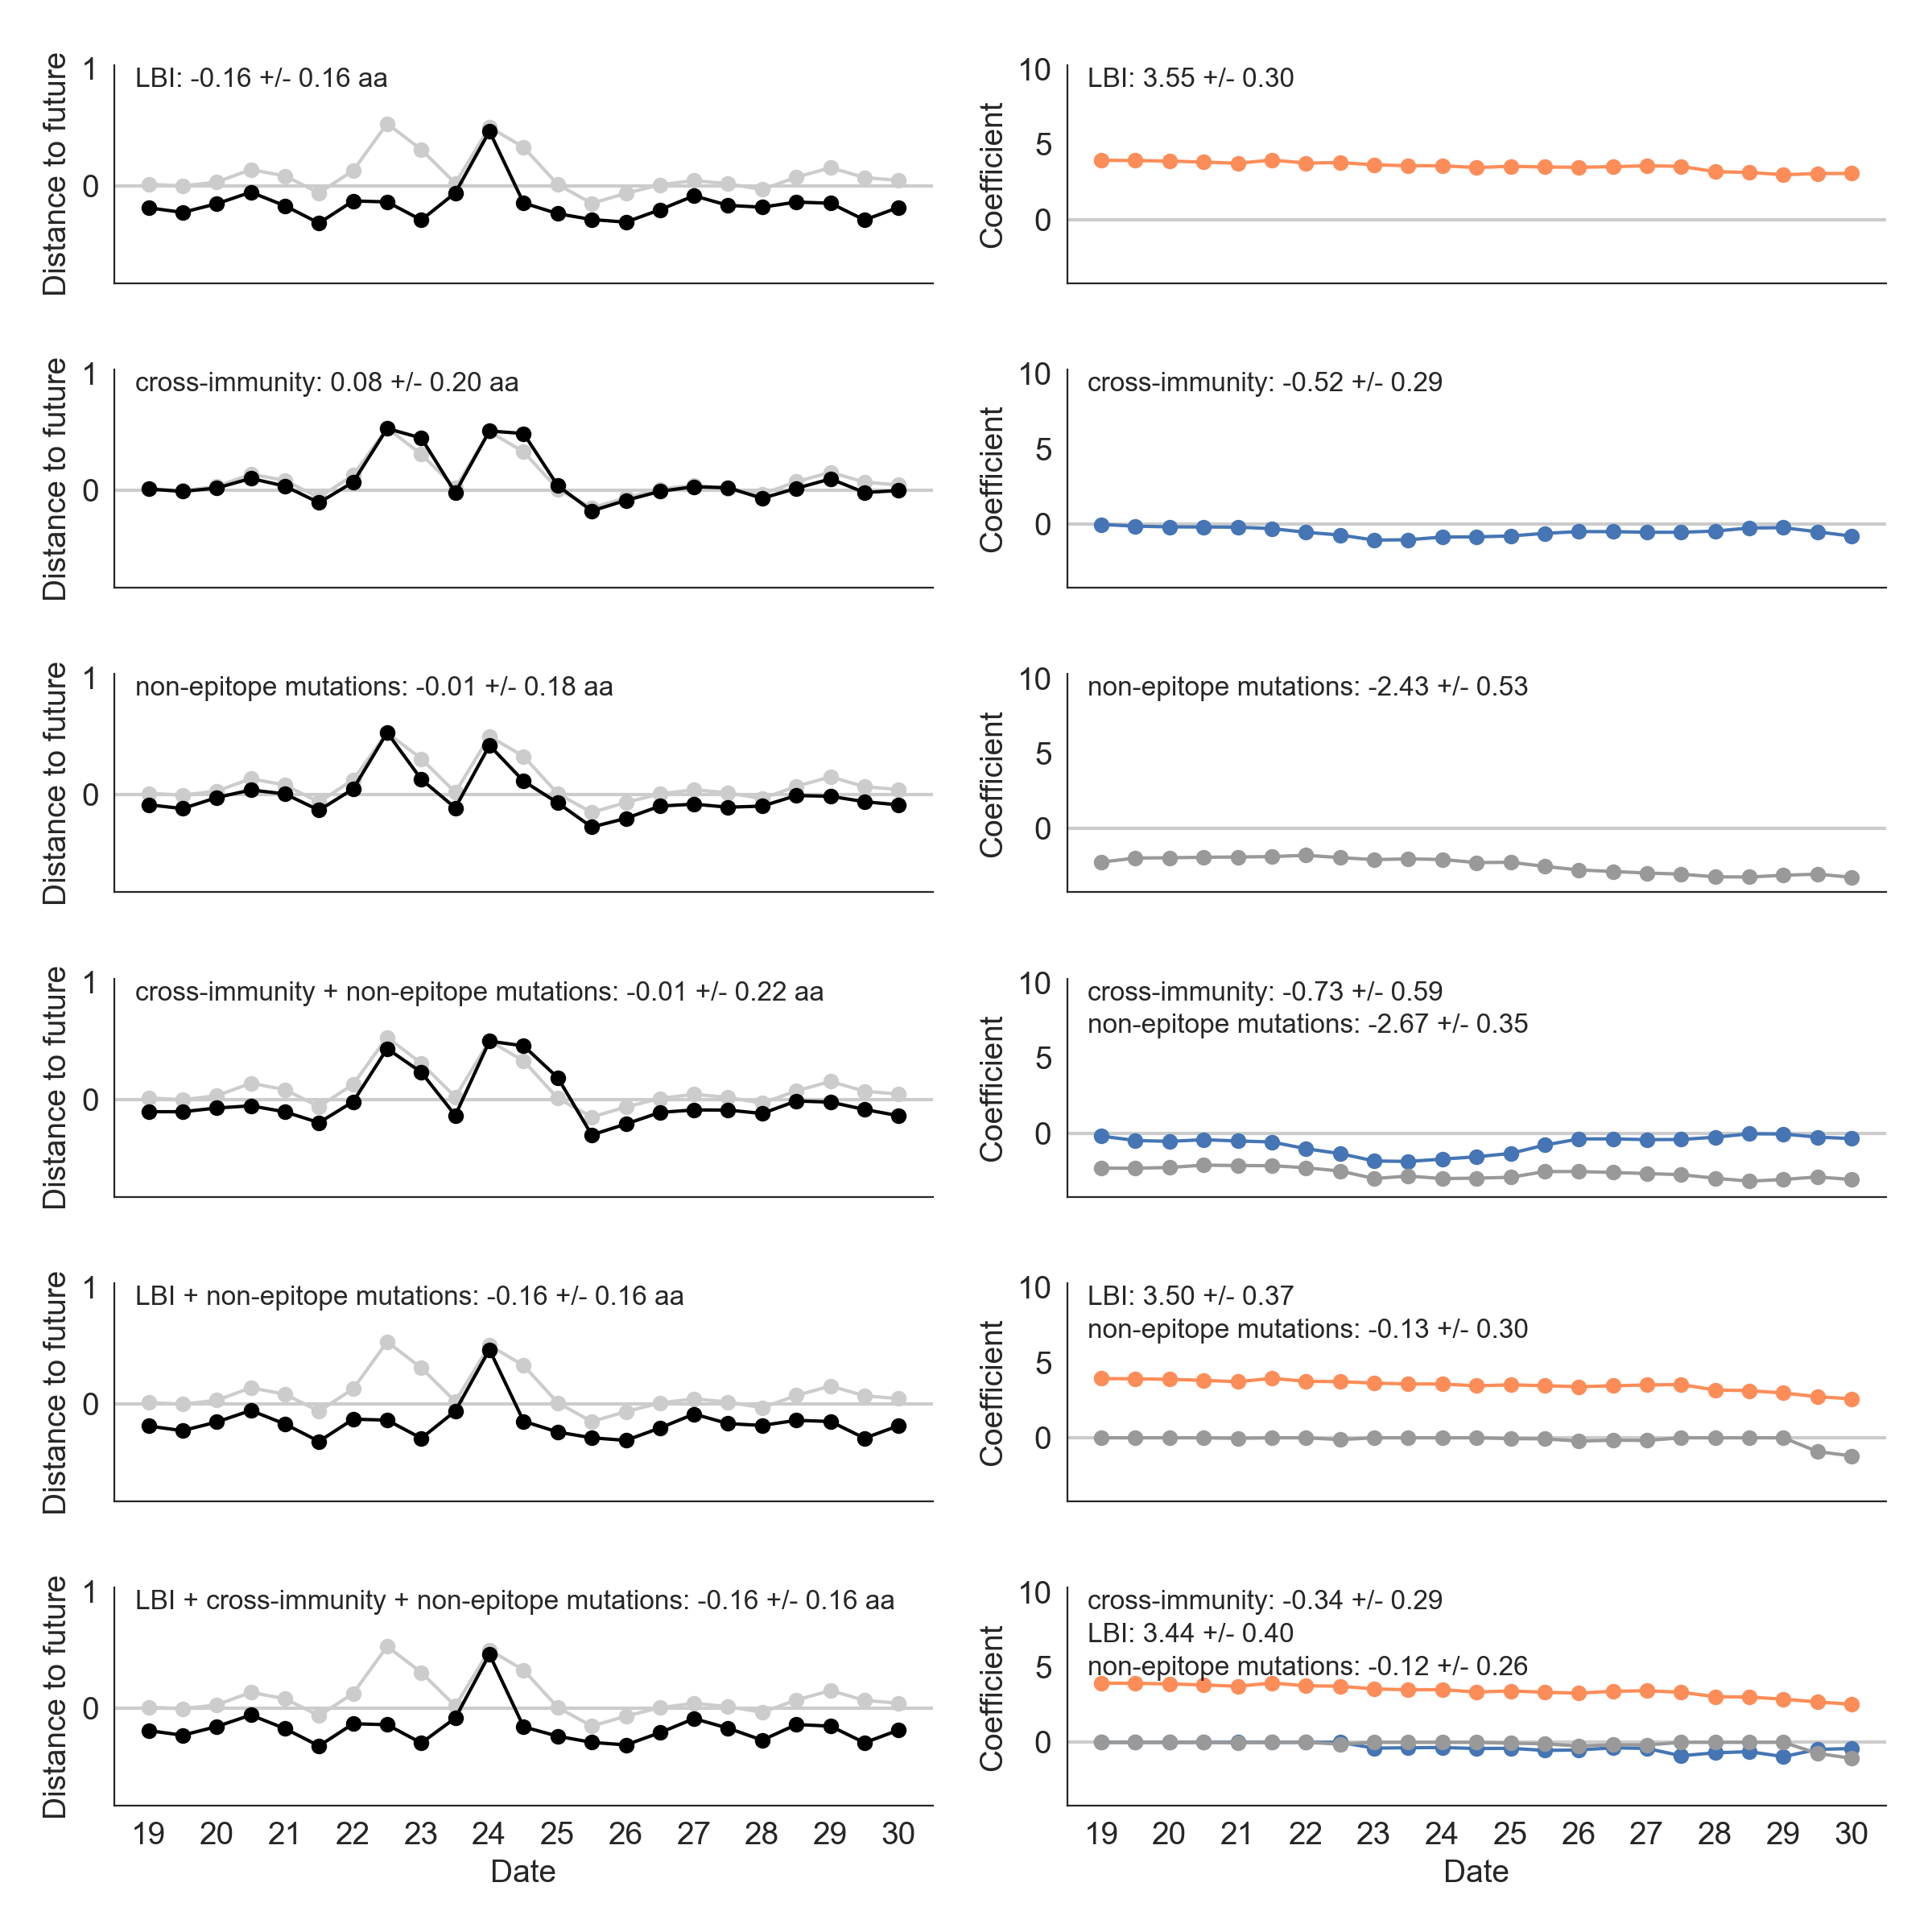
\includegraphics[width=\textwidth]{figures/unadjusted-composite-model-accuracy-and-coefficients-for-simulated-populations.png}
  \caption{Composite model a) accuracy and b) coefficients for simulated populations of A/H3N2-like viruses.}
  \label{sup_fig:unadjusted_composite_model_accuracy_and_coefficients_for_simulated_populations}
  \end{center}
\end{figure*}

\begin{figure*}[t]
  \begin{center}
  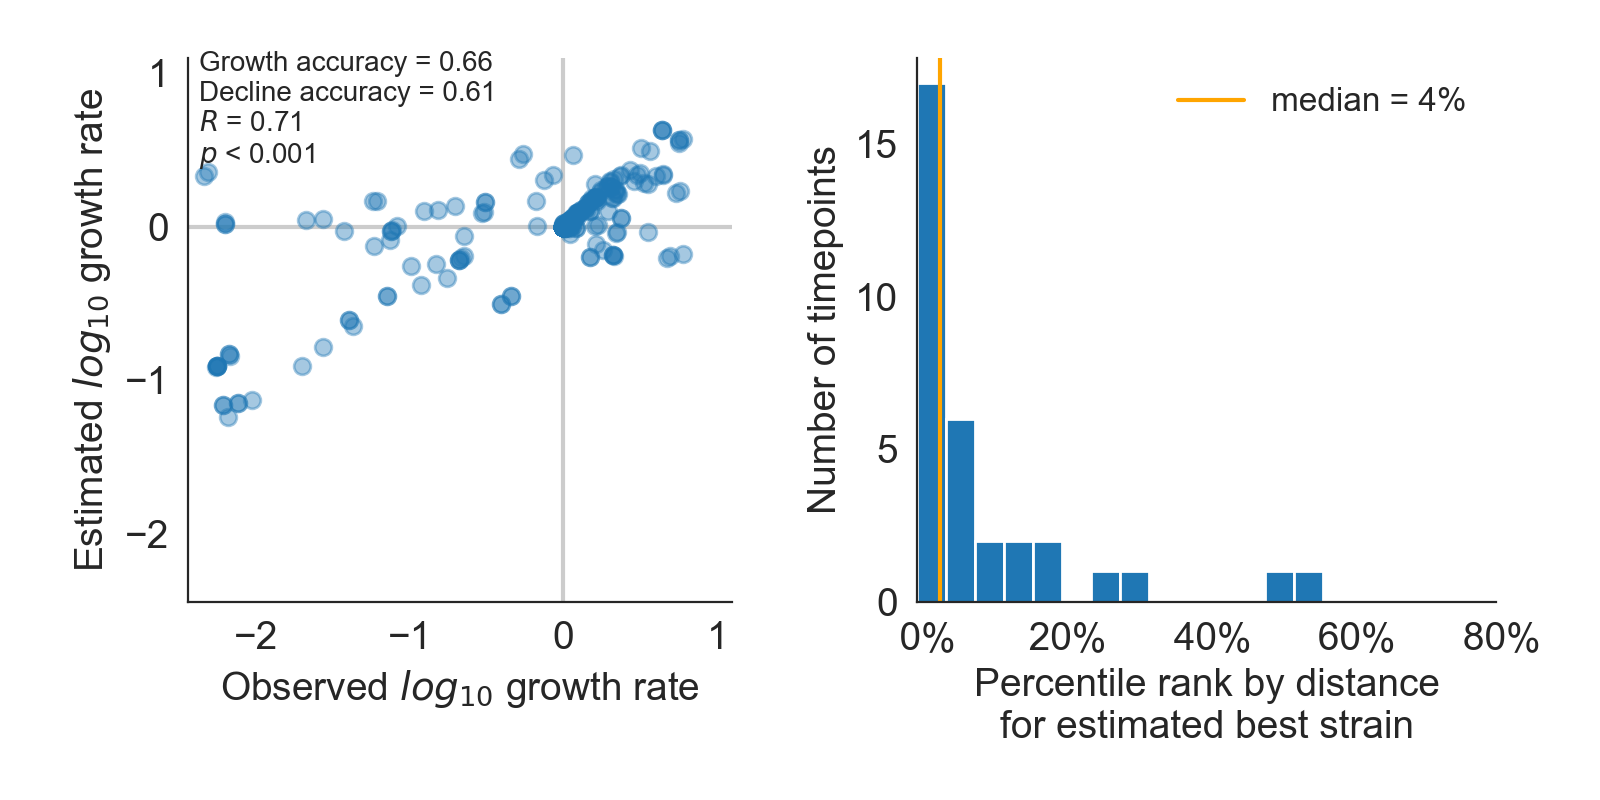
\includegraphics[width=\textwidth]{figures/validation-of-best-model-for-simulated-populations.png}
  \caption{
  Validation of best model for simulated populations of A/H3N2-like viruses.
  a) The correlation of estimated and observed clade growth rates shows the model's ability to capture clade-level dynamics without explicitly optimizing for clade frequency targets.
  b) The rank of the estimated best strain based on its distance to the future in the best model shows how often the model makes a good choice when forced to select a single representative strain for the future population.
  }
  \label{sup_fig:validation_of_best_model_for_simulated_populations}
  \end{center}
\end{figure*}

\begin{table*}[ht]
  \begin{center}
    \begin{tabular*}{1.0\textwidth}{lrrrl}
\toprule
                             Model & Coefficients & \makecell{Distance to \\ future (AAs)} & \makecell{Approx. of future \\ diversity (AAs)} & \makecell[l]{Model $>$ naive \\ (N=20)} \\
\midrule
                             LBI + &         1.31 &                          7.09 +/- 1.15 &                                  -1.28 +/- 1.96 &                               19 (95\%) \\
 \hspace{3mm}non-epitope mutations &        -1.77 &                                        &                                                 &                                         \\
                      true fitness &         9.37 &                          7.32 +/- 1.80 &                                  -0.32 +/- 2.38 &                               18 (90\%) \\
                               LBI &         2.26 &                          7.58 +/- 1.15 &                                  -1.36 +/- 1.96 &                               17 (85\%) \\
          epitope cross-immunity + &         0.42 &                          8.00 +/- 1.63 &                                   0.53 +/- 2.25 &                               17 (85\%) \\
 \hspace{3mm}non-epitope mutations &        -1.60 &                                        &                                                 &                                         \\
                epitope ancestor + &         0.35 &                          8.01 +/- 1.53 &                                   0.54 +/- 2.19 &                               19 (95\%) \\
 \hspace{3mm}non-epitope mutations &        -1.57 &                                        &                                                 &                                         \\
             non-epitope mutations &        -1.49 &                          8.04 +/- 1.51 &                                   0.58 +/- 2.26 &                               19 (95\%) \\
                   delta frequency &         1.46 &                          8.51 +/- 1.93 &                                   0.89 +/- 2.49 &                               15 (75\%) \\
                  epitope ancestor &         0.14 &                          8.85 +/- 1.68 &                                   1.77 +/- 2.39 &                               14 (70\%) \\
                             naive &         0.00 &                          8.90 +/- 1.69 &                                   1.80 +/- 2.43 &                                 0 (0\%) \\
            epitope cross-immunity &         0.02 &                          8.90 +/- 1.70 &                                   1.80 +/- 2.43 &                               13 (65\%) \\
\bottomrule
\end{tabular*}

    \caption{
      Model coefficients and test performance for simulated populations ordered from best to worst by distance to the future.
      Coefficients shown here are the mean values across all training and validation windows which were used to test models on out-of-sample data.
      Distance to the future, approximation of future diversity, and number of times model outperforms the naive model are as in Table~\ref{table_simulated_model_selection} for all test timepoints (N=20).
    }
    \label{table_simulated_model_test}
  \end{center}
\end{table*}

\begin{figure*}[h]
  \begin{center}
  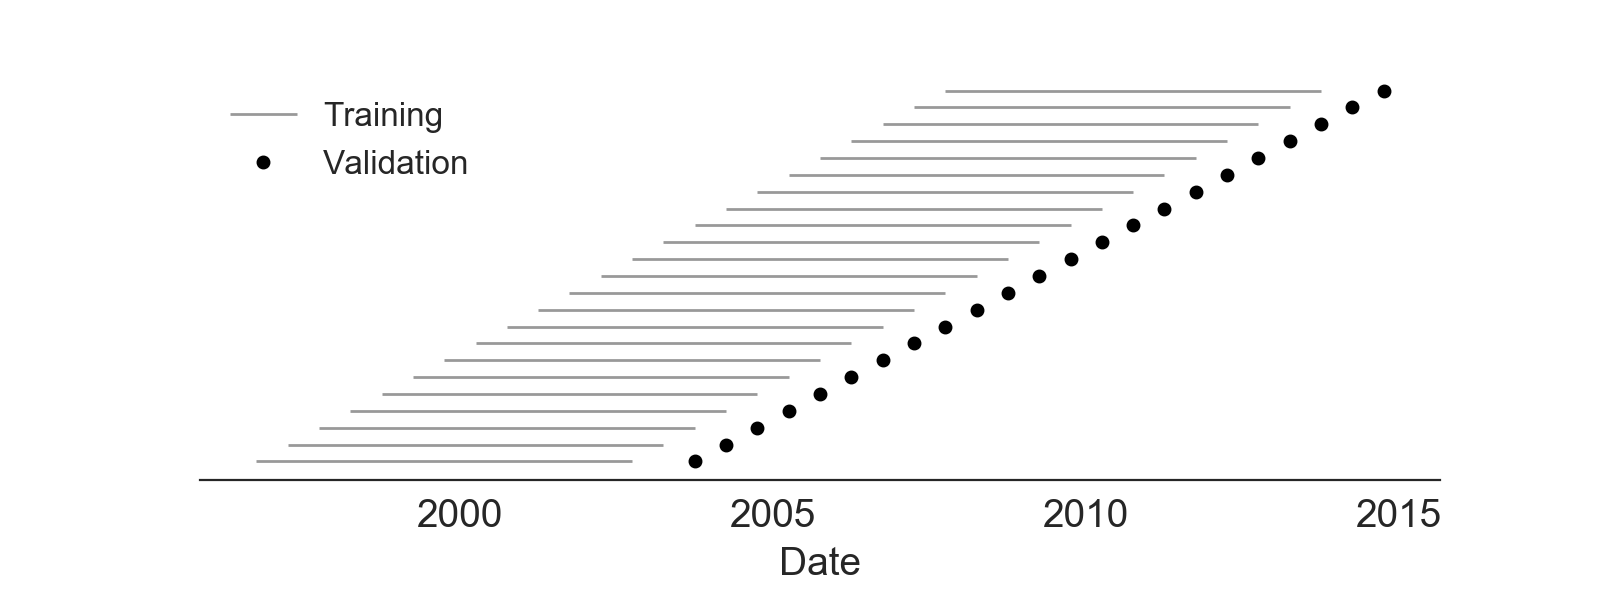
\includegraphics[width=\textwidth]{figures/cross-validation-for-natural-populations.png}
  \caption{
  Time-series cross-validation scheme for natural populations.
  Models were trained in six-year sliding windows (grey lines) and validated on out-of-sample data from validation timepoints (filled circles).
  Validation results from 25 years of data were used to iteratively tune model hyperparameters.
  After fixing hyperparameters, model coefficients were fixed at the mean values across all training windows.
  Fixed coefficients were applied to four years of new out-of-sample test data (open circles) to estimate true forecast errors.
  }
  \label{sup_fig:cross_validation_for_natural_populations}
  \end{center}
\end{figure*}

\begin{table*}[ht]
  \begin{center}
    \begin{tabular}{lll}
\toprule
                                           Model & \makecell{Distance closer \\ to future (AAs)} & \makecell{Model $>$ naive \\ (N=23)} \\
\midrule
                     non-epitope mutations + LBI &                                 0.96 +/- 1.42 &                            18 (78\%) \\
                                             LBI &                                 0.72 +/- 1.51 &                            17 (74\%) \\
       HI cross-immunity + non-epitope mutations &                                 0.63 +/- 0.79 &                            18 (78\%) \\
 HI cross-immunity + non-epitope mutations + LBI &                                 0.52 +/- 0.83 &                            19 (83\%) \\
                                         HI tree &                                 0.40 +/- 0.82 &                            15 (65\%) \\
                               HI cross-immunity &                                 0.36 +/- 0.65 &                            17 (74\%) \\
                                 delta frequency &                                 0.27 +/- 0.67 &                            16 (70\%) \\
                           non-epitope mutations &                                 0.26 +/- 0.56 &                            17 (74\%) \\
                          Koel epitope mutations &                                 0.19 +/- 0.25 &                            19 (83\%) \\
                                     DMS entropy &                                 0.02 +/- 0.15 &                            14 (61\%) \\
                                 DMS non-epitope &                                -0.05 +/- 0.15 &                             7 (30\%) \\
                        linear HI mut phenotypes &                                -0.06 +/- 0.51 &                            11 (48\%) \\
                           HI sub cross-immunity &                                -0.14 +/- 0.57 &                            10 (43\%) \\
                          Wolf epitope mutations &                                -0.17 +/- 0.31 &                             5 (22\%) \\
                          DMS mutational effects &                                -0.35 +/- 1.65 &                            11 (48\%) \\
                               epitope mutations &                                -0.43 +/- 0.94 &                             5 (22\%) \\
  epitope cross-immunity + non-epitope mutations &                                -0.54 +/- 1.39 &                             6 (26\%) \\
                          epitope cross-immunity &                                -0.66 +/- 1.13 &                             6 (26\%) \\
\bottomrule
\end{tabular}

    \caption{
      All model coefficients and validation performance for natural populations ordered from best to worst by distance to the future, as in Table~\ref{table_simulated_model_selection}.
      Results are based on training and validation across 23 training windows.
      Model results for additional variants of fitness metrics including those based on epitope mutations and DMS preferences are included for reference.
    }
    \label{sup_table:complete_natural_model_selection}
  \end{center}
\end{table*}
